\documentclass{article} % For LaTeX2e
\usepackage{iclr2017_conference,times}
\usepackage{url}
\usepackage{amsthm}
\usepackage{times}
\usepackage{graphicx}
\usepackage{color}
\usepackage{amsmath}
\usepackage{amsfonts}
\usepackage{url}
\usepackage{textcomp}
\usepackage{amsthm}
\usepackage{float}

\frenchspacing

\def\presentationmode{1}

\def\beginFrame#1{\if\presentationmode1 \begin{frame}{#1} \else \fi}
\def\endFrame{\if\presentationmode1 \end{frame} \else \fi}

\newcommand{\mat}[1]{\mathrm{\mathbf{#1}}}
\newcommand{\vect}[1]{\mathrm{\mathbf{#1}}}
\newcommand{\fros}[1]{\left\| #1 \right\|_\mathrm{F}^2}
\newcommand{\Expect}[2]{\mathbb{E}_{#1}\left[ #2 \right]}
\newcommand{\KL}[2]{ \mathrm{KL}\left( #1 \| #2 \right) }
\newcommand{\Real}{\mathbb{R}}
\newcommand{\T}{\mathrm{T}}
\newcommand{\tr}{\mathrm{tr}}
\newcommand{\sigmoid}{\sigma}
\newcommand{\Simga}{\Sigma}
\newcommand{\attention}{\vect{g}}
\def\attentionwithouti{g_2, \dots, g_k}
%\def\attentionwithouti{\boldsymbol{\gamma}_{i}}
\newcommand{\attraction}{\vect{h}}

\def\x{\vect{x}}
\def\y{\vect{y}}
\def\h{\vect{h}}
\def\g{\vect{g}}
\def\s{\vect{s}}
\def\c{\vect{c}}
\def\A{\mathcal{A}}
\def\S{\mathcal{S}}
\def\R{\mathcal{R}}
\def\Trans{\mathcal{T}}
\def\E{\mathcal{E}}
\def\deriv#1#2{ \frac{\partial #2}{ \partial #1 } }
\def\derivN#1#2#3{ \frac{\partial^{#1} #3}{ \partial #2^{#1} } }
\def\grad#1#2{ \deriv{#1}{#2} }
\def\gradN#1#2#3{ \derivN{#1}{#2}{#3} }
\def\Grad#1#2{ \nabla_{#1} {#2} }
\def\obs{\vect{o}}
\def\u{{\boldsymbol{b}}}
\def\w{{\boldsymbol{\alpha}}}
\def\vmu{{\boldsymbol{\mu}}}
\def\v{\vect{v}}
\def\g{\attention}
\def\h{\attraction}
\def\G{\mat{G}}
\def\op{}
%\def\Qg{Q^{\mathrm{g}}}
%\def\ug{\vect{u}^{\mathrm{g}}}
\def\Qg{Q}
\def\ug{\u}
\def\params{{\boldsymbol{\theta}}}
\def\Params{{\boldsymbol{\Theta}}}
\def\opt#1{{\hat{#1}}}
\def\argmax{\mathrm{argmax}}

%\def\costof#1{C(#1)}
\def\costof#1{\mathrm{C}[{#1}]}
\def\budget{B}
\def\cost{c}
\def\vcost{\vect{\cost}}
\def\costat#1{\cost_{#1}}
\def\costi{c_i}
\def\unit{\vect{e}}
\def\units{k}
\def\state{\s}
\def\action{a}
\def\rewards{y}

\def\sumk#1{\sum_{#1=1}^k}
\def\Si{\sumk{i}}
\def\Sj{\sumk{j}}

\def\vcatout{\tilde{\vect{h}}}
\def\catout{\tilde{h}_i}
\def\catoutj{\tilde{h}_j}
\def\changeof#1{\Delta #1}

\def\vcatin{\vect{h}}
\def\catin{h_{i}}
\def\catinj{h_{j}}

\def\vcatbias{\vect{h}_i}
\def\catbias{\mu_i}
\def\catbiasj{\mu_j}

\def\qbias{q_i}
\def\vqbias{\mathbf{q}}
\def\qin{Q}

\def\ebias{e_{-i}}
\def\ein{e}
\def\changeofebias{{\changeof\qbias} \left[ \changeof\qbias + 2 \TDerror{\qin} \right]}
%\def\changeofebias{{\changeof\qbias}\left( \changeof\qbias + 2 \delta_t \right)}

\def\regret{\rho_{-i}}
%\def\TDerror#1{E_{\mathrm{TD}}\left({#1}\right)}
\def\TDerror#1{\delta}


\def\prA{p(\rewards|\state, \action, \params, \g)}
\def\LLAttention{\log \prA}

\def\Square#1{\left[ #1 \right]^2}

\def\ReplayMemory{\mathcal{D}}
\def\play{\s_t, a_t, r_t, \s_{t+1}}
\def\Play{(\play)}
\def\pl{\mathsf{d}_t}
\def\Replays#1{\Expect{ \pl \sim \ReplayMemory}{#1}}

\def\bUpdate#1{p(o_{t+1}|s_${#1},a_t) \sum_i p(s_{#1}|s_i, a_t) b_{t}^i}
\def\beliefState#1{ \vect{b}_{#1} }

\def\const{\mathrm{const.}}
\def\test{_\mathrm{test}}
\def\train{_\mathrm{train}}
\def\bs{\boldsymbol}
\def\etal#1{{et al.} (\citeyear{#1})}
\def\Etal{{et al.}}
\def\Long{1}
\def\eg{e.g., }

\def\eAt#1{e_{#1}}
\def\eBase{\eAt{\one}}
\def\one{\mathbf{1}}
\def\zero{\mathbf{0}}
\def\unit#1{\vect{u}_{#1}}
\def\eChange#1{ \Delta e_{#1} }

\def\ask{q}


% probability
\def\prob#1{p\left(#1\right)}
\def\prob#1#2{p\left(#1 \mid #2 \right)}

\def\deprecated{\alert{[Deprecated]}}
\def\softmax{\mathrm{softmax}}


\newcommand{\penalvec}[3]{ \frac{1}{2 \sigma_#1^2} \sum_{#2=1}^{#3} \vect{#1}_{#2}^\T  \vect{#1}_{#2} }

\newcommand{\CON}{\color{red}}
%\newcommand{\CON}{\color{black}}
\newcommand{\COFF}{\color{black}}

%\newcommand{\CON}{\color{red} -------- My modification starts from here. ------- \color{black}}
%\newcommand{\CON}{\color{black}}
%\newcommand{\COFF}{\color{red} -------- My modification ends here. ------- \color{black} }


\newtheorem{thm}{Theorem}[section]
\newtheorem{coro}{Corollary}[section]
\newtheorem{prf}{Proof}
\newtheorem{defn}{Definition}



\title{Neuron as an Agent}

%\author{Shohei Ohsawa, Kei Akuzawa, Yusuke Iwasawa \& Yutaka Matsuo \\
%The University of Tokyo\\
%7 Chome-3-1 Hongo, Bunkyo, Tokyo \\
%\texttt{ohsawa@weblab.t.u-tokyo.ac.jp} \\
%}
\author{Anonymous}

\newcommand{\fix}{\marginpar{FIX}}
\newcommand{\new}{\marginpar{NEW}}

\begin{document}

\maketitle

\begin{abstract}
%The reason why swarm of agents solve real-world problem well is, interestingly,
%same as the principle of representation learning: good representation improves
%perforamance of machine learning. Most of the problem in real-world is not
%Markov decision process (MDP) but partially observed MDP (POMDP). On the
%POMDP environment, good observation yields good action. In this paper, we
%optimise a deep neural network as a multi-agent system as a natural extension
%from representation learning to multi-agent reinforcement learning for POMDP.
%To achieve that, we propose a novel learning framework, neuron as an agent
%(NaaA). In NaaA, an individual unit is considered as an agent, and they maximizing
%profit instead of minimizing error. To prevent dillemma, we borrow idea
%from machanism design, a field of game theory. To this end, we show all the unit
%have valid price reflecting their contribution to performance at convergence. We
%confirm the result by numerical experiment using Atari and VizDoom.
\end{abstract}

\section{Introduction}
Deep reinforcement learning (DRL) succeeds in many areas.
Deep Q-Network (DQN) \citep{mnih2015human,silver2016mastering} finds the optimal action from a screen sequence from Atari, and selects the move closest to win from a face of a board of Go.
Deep Deterministic Policy Gradient (DDPG) \citep{lillicrap2015continuous} realizes the multiple-join control considering conditions such as friction and gravity factors in a physical space.
The applicability of DRL is becoming wider year by year. Reasonable performance is reported for 3D games such as Doom \citep{dosovitskiy2016learning}.

A neural network is workable for DRL because a neural network abstracts the implicit state in an environment and obtains an informative state representation.
From a micro perspective, the abstraction capability of each unit contributes to the return of the entire system.
Therefore, we address the following question.

\begin{center}
{\em Will reinforcement learning work even if we consider each unit as an autonomous agent?}
\end{center}

The contribution of this paper is that we propose {\em Neuron as an Agent} (NaaA) as a novel framework for RL, and its optimization method.
NaaA incorporates all neural network units as agents and optimizes the reward distribution as a multi-agent RL problem.
In the of NaaA reward design, a unit distributes its received reward to other input units, passing its activation to the unit as cost.
Consequently, the actual reward is profit, defined as the difference between inflow (received reward) and outflow (paid cost).
In the setting, the economic metaphor can be introduced: profit is the balance of revenue and cost. 
Therefore, a unit should address tradeoffs between optimization of cumulative revenue maximization and cumulative cost minimization.

This paper is organized as presented below.
First, showing the optimization of NaaA, this report describes the negative result that the performance decreases if we naively consider units as agents.
As a solution to this difficulty, we introduce a mechanism of auction which applies game theory.
As a theoretical result, we demonstrate that the agent obeys to maximize its {\em counterfactual return} as the Nash equilibrium.
The counterfactual return is that by which we extend counterfactual reward, the criterion proposed for multi-agent reward distribution problem \citep{agogino2006quicr}, along a long time axis.

Subsequently, we present that learning counterfactual return leads the model to learning optimal topology between the units.
In addition, we propose {\em adaptive dropconnect}, a natural extension of dropconnect \citep{wan2013regularization}.
Adaptive dropconnect combines dropconnect, which pure-randomly masks the topology, with adaptive algorithm, which prunes the connection with less counterfactual return with higher probability.
It uses $\varepsilon$-greedy as a policy, and is equivalent to dropconnect in the case of $\varepsilon = 1$. It is equivalent to counterfactual return maximization, which constructs the topology deterministically in the case of $\varepsilon = 0$.

Finally, we confirm that optimization with the framework of NaaA leads to better performance of RL, with numerical experiments.
Specifically, we use a single-agent environment from Open AI gym, and a multi-agent environment from ViZDoom.

Although considering all the units as agents might be simplistic at first glance, it has a wider applicable area.
From the perspective of optimization for a single neural network, it can be applied to pruning by optimizing the topology.
Furthermore, introducing the concept of reward distribution divides the single neural network to numerous autonomous parts.
It enables us not only to address sensor placing problem in IoT for partially observed Markov decision process (POMDP): arbitrary incentivized participants can join the framework.
 

\section{Related Work}
NaaA belongs to a class of partially observable stochastic game (POSG) \citep{hansen2004dynamic} because it processes multiple units as agents.
POSG, a class of reinforcement learning with multiple agents in a POMDP environment, presents several research issues, one of which is communication.
CommNet \citep{sukhbaatar2016learning}, which exploits the characteristics of a unit that is agnostic to the topology of other units, employs backpropagation to train multi-agent communication.
Another one is credit assignment.
Instead of reward $R(a_t)$ of an agent $i$ for actions at $t$ $a_t$, 
QUICR-learning \citep{agogino2006quicr} maximizes counterfactual reward $R(a_t) - R(a_t - a_{it})$, the difference in the case of the agent $i$ takes an action $a_{it}$ ($a_t$) and not ($a_t-a_{it}$).
COMA \citep{foerster2017counterfactual} also maximizes counterfactual rewards in an actor--critic setting.
In the setting, all actors have common critics, which improves both actors and critics with time difference (TD)-error of a counterfactual reward.
This paper unifies both issues: communication and credit assignment.
The main proposal is a framework to manage the agents to maximize the {\em counterfactual return}, the extended counterfactual reward along the time axis.

Training a neural network with a multi-agent game is an emerging methodology.
Generative adversarial nets (GAN) \citep{goodfellow2014generative} have the goal of obtaining true generative distribution as a Nash equilibrium of a competitive game that includes two agents with contradictory rewards: a generator and a discriminator. 
In game theory, the outcome maximizing overall reward is named Pareto optimality.
Nash equilibrium is not guaranteed to converge to Pareto optimality. The difference between them is designated as a dilemma.
Because the existence of a dilemma depends on the reward design, methods to resolve dilemmas with good reward design are being investigated: mechanism design \citep{myerson1983mechanism} is also known as inverse game theory.
Mechanism design is applied to auctions \citep{vickrey1961counterspeculation} and matching \citep{gale1962college}.
GAN and our proposal, NaaA, are outcomes from mechanism design.
NaaA applies a digital goods auction \citep{guruswami2005profit} to reinforcement learning with a multi-agent neural network, 
to obtain a maximized return by units as a Nash equilibrium.

Adaptive DropConnect (ADC) which we propose in a late part of this paper, extends DropConnect \citep{wan2013regularization}, a regularization technique.
The idea of ADC (instead of dropping each connection between the units in constant probability, using skew probability correlated to absolute value of weights) is eventually closer to Adaptive DropOut \citep{ba2013adaptive} although the derivation is different, 
and the adjective ``adaptive'' is added respecting the method.
Optimizing neural network with RL is investigated by \cite{andrychowicz2016learning}.
In contrast to their methods which uses recurrent neural network (RNN) and hence the implementation is difficult,
our method is RNN-free and forms as a layer, and hence the implementation is easy and fast, and it has wide applicable area.

\section{Background}
First, we consider a POMDP environment in which a single agent acts.
The POMDP environment is a seven-tuple $(\S, \A, \Trans, \R, \Observations, \ObProb, \gamma)$,
where $\S$ represents a set of states, $\A$ stands for a set of actions, $\Trans$ denotes a transitive probability, 
$\R: \S \times \A \rightarrow \Real $ is a function from the state and the action of an agent to the real value.
$\Observations$ represents a possible set of observations, $\ObProb$ denotes a set of observation probability, and
$\gamma$ is the discount rate.
An agent partially predicts state $h \in \S$ through an observation $s \in \Observations$.

Generally, $s$ has higher dimensions than $h$, and is complex.
For example, although Atari 2600 has a read only memory (RAM) as the true state, which contains 128 bytes,
the generated image from that $s$ has more than 10,000 dimensions.
Therefore, DQN and DRQN abstract $s$, and create original state representation to predict good action efficiently.
(Although the original paper of DQN assumes MDP, the paper of DRQN pointed out that the environment is POMDP).
Although DQN does not address the state transition directly because it is model-free method, 
some interpretations hold that the hidden state representation is learned in the previous layer of the output layer \citep{zahavy2016graying}
Using the method below, we assume that the agent chooses an action through a neural network.
The POSG environment is a natural extension of POMDP to multi-agent environment defined by a tuple $(\S, \A^i, \Trans, \R^i, \Observations^i, \ObProb^i, \gamma^i)_{i \in \mathcal{I}}$,
where $\mathcal{I}$ is a finite set of agents indexed 1, \dots, $N$.
Each agent has a policy $\pi_i: \Observations^i \rightarrow \A^i$. 
They maximize their return by interacting with the environment.

%The POSG environment is a multi-agent environment defined by a tuple $(\S, \A^i, \Trans, \R^i, \Observations^i, \ObProb^i, \gamma^i)_{i \in \mathcal{I}}$,
%where $\mathcal{I}$ is a finite set of agents indexed 1, \dots, $N$, 
%$\S$ represents a set of states, 
%$\A^i$ stands for a set of actions, 
%$\Trans$ denotes a transitive probability, and 
%$\R^i: \S \times \A^1 \times \cdots \times \A^N \rightarrow \Real $ is a function from the state and the action of all agents to the real value.
%$\Observations^i$ represents a possible set of observations. $\ObProb^i$ denotes a set of observation probability.
%$\gamma^i$ is the discount rate.
%Each agent has a policy $\pi_i: \Observations^i \rightarrow \A^i$. They maximize their return by interacting with the environment.
%A difference from POMDP is that there are $N$-agents.

We employ several concepts from game theory.
Although RL and game theory are typically investigated in parallel, several concepts in game theory can be written in the domain of RL.
The (Bayesian) Nash equilibrium $\hat{\pi}_{i}$ is a policy by which all agents maximize their expected reward. That is,
\begin{flalign}
\hat{\pi}(s_{it}) = \argmax_{a_i \in \A^i} \Expect{ \vect{a}_{-i} \in A^{-i}, h \sim \ObProb^i }{ \R^i(h, \vect{a}) | s_{it}} \, \forall i \in \mathcal{I},
\end{flalign}
where $\mathcal{A}^{-i}$ is a set of actions except for $i$. 
Intuitively, the equation took an expected value of reward to integrate out other agents' unobserved actions.
Because the Nash equilibrium is sufficient to state only the best action in the most cases, we use the notation with action $\hat{\vect{a}}$ in the following.


\section{Neuron as an Agent}
%TODO: Show the figure.
% ���̏͂ł�������
% �E�j���[�������G�[�W�F���g�Ƃ݂Ȃ�
% �E�����‚��̑O����Ă���
% �ENaaA �� social welfare function ���ő剻���邱�Ƃ��A�O������̃����[�h�ő剻�Ɉ�v����B

\subsection{Problem Definition}
Suppose there are $N$ agents interacting to an environment. 
%This paper addresses reward distribution problem at multi-agent communication among the agents.
Some agents get reward from the environment, and distribute it to other agents as incentive to give precise information.
The reward is limited so that if an agent distribute $\rho$ reward, the agents' reward subtracted by $\rho$ such as currency.
For the reason, other agents for an agent itself can be interpreted as another environment which 
give a reward $-\rho$ instead of an observation $x$.
We name the another environment as {\em internal environment} and name the original environment as an {\em external environment}.

Our goal is to maximize the discounted cumulative reward which the system will obtain from the external environment.
 %total discounted cumulative reward from the external environment which all the $N$ agents will obtain.
\begin{equation}
%G^\mathrm{ex} = \sum_{i=1}^n \left[ \sum_{k=0}^T \gamma^k R_{i,k+t}^\mathrm{ex} \right],
G = \sum_{i=1}^n \left[ \sum_{t=0}^T \gamma^k R_{it}^\mathrm{ex} \right],
\end{equation}
where $R_{it}^\mathrm{ex}$ is an external reward which $i$-th agent obtains at $t$, and $\gamma \in [0, 1]$ is the discount rate and $T$ is the terminal time.

Similarly to CommNet \citep{sukhbaatar2016learning}, we assume that the communication protocol between the agent is a continuous quantity such as a vector, and the content can be trained by backpropagation.
Hence, we can interpret the multi-agent communication as a huge neural network.
Therefore, we can interpret a unit as an agent without loss of generality.
This framework can single-agent reinforcement learning as well as multi-agent reinforcement learning.

\subsection{The Framework}
A typical artificial neural network is a directed graph $\neuralnet = (\units, \edges)$ among the units.
$\units = \{\unitAt{1}, \dots, \unitAt{N}\}$ is a set of the units. $\edges \subset \units^2$ is a set of edges representing connections between two units.
If $(\unit, \unitAt{j}) \in \edges$, then connection $\unit \rightarrow \unitAt{j}$ holds, indicating that $\unitAt{j}$ observes activation of $\unit$.
We denote activation of the unit $\unit$ at time $t$ as $x_{it} \in \Real$.
Additionally, we designate a set of units which unit $i$ connects to as $\followers = \{j | (\unit, \unitAt{j}) \in \edges \}$ and a set of units which unit $i$ is connected from as $\followees = \{j | (\unitAt{j}, \unit) \in \edges \}$.
We denote $\friends = \followees \cup \followers$.

NaaA interprets $\unit$ as an agent.
Therefore, $\neuralnet$ is a multi-agent system.
An environment for $\unit$ comprises an environment that the multi-agent system itself touches and a 
set of the unit to which $\unit$ directly connects: $\{v_i \in \units | i \in \friends\}$.
We distinguish both environments by naming the former as an external environment, and by naming the latter as an internal environment.
$\unit$ will receive rewards from both environments.
We add the following assumption for characteristics of the $\unit$.
\begin{enumerate}
\renewcommand{\labelenumi}{N\arabic{enumi}:}
\item (Selfishness) 
	The utility which an $\unit$ wants to maximize is its own return (cumulative discounted reward):
	$G_{it} = \sum_{k=0}^T \gamma^k \rewardAt{i,t+k}$.
\item (Conservation) 	% Energy Conservation
	The summation of internal reward over $\units$ equals to 0.
	Hence, the summation of a reward by which $\units$ will receive both an internal and external environment $\reward$ are equivalent to reward $R_t^{\mathrm{ex}}$, which the entire multi-agent system receives from the external environment.
\item (Trade) 
	The $\unit$ receives internal reward $\rho_{jit}$ from $\unitAt{j} \in \units$ in exchange of activation signal $x_i$
	before transferring the signal to the unit. At the same time, $\rho_{jit}$ is subtracted from the reward of $v_j$.
\item (NOOP) 
	$\unit$ has NOOP (no operation), for which the return is $\delta > 0$ as an action.
	With NOOP, the unit inputs nothing and outputs nothing.
\end{enumerate}
In terms of neuroscience,
N1 states that the unit acts as a cell.
N2 and N3 state the distribution of NTF. N4 corresponds to apoptosis.
NOOP is selected when the expected returns of the other actions are non-positive.
In the following, we construct the framework of NaaA from the assumptions.

The social welfare function (total utility of the agents) $G^\mathrm{all}$ is equivalent to the objective function $G$. That is,
\begin{equation}
	G^\mathrm{all} = \sum_{i=1}^n G_{it} = \sum_{i=1}^n \left[ \sum_{k=0}^T \gamma^k R_{it} \right] 
		= \sum_{k=0}^T \left[ \gamma^k \sum_{i=1}^n R_{it} \right].
\end{equation}
From N2, $\sum_{i=1}^n R_{it} = \sum_{i=1}^n R_{it}^{\mathrm{ex}}$ holds. Hence, $G^\mathrm{all} = G$ holds.
%\begin{equation}
%	G^\mathrm{all} = \sum_{k=0}^T \left[ \gamma^k \sum_{i=1}^n R_{it}^{\mathrm{ex}} \right] = G.
%\end{equation}

%================================================================
\subsection{Cumulative Discounted Profit Maximization Framework}
%================================================================
We denote the external reward by which unit $\unit$ receives at time step $t$ as $R_{it}^\mathrm{ex}$, where $\sum_{i=1}^n R_{it}^\mathrm{ex} = R_t^{\mathrm{ex}}$ holds.
From N3, reward $R_{it}$, which $\unit$ receives at $t$ can be written as the following.
\begin{flalign}
	R_{it} = 
	  R_{it}^\mathrm{ex} + \sum_{j \in N^\mathrm{out}_i} \rho_{jit} 
	- \sum_{j \in N^\mathrm{in}_i} \rho_{ijt}.
\end{flalign}
The equation is divided into positive terms and a negative term, we name the former as revenue, and the latter as cost, and denote them respectively as $r_{it} = R_{it}^\mathrm{ex} + \sum_{j \in N^\mathrm{out}_i} \rho_{jit}, \, c_{it} = \sum_{j \in N^\mathrm{in}_i} \rho_{ijt}$.
We name $R_{it}$ as profit.


$\unit$ maximizes the cumulative discounted profit $G_{it}$ represented as
\begin{flalign}
	G_{it}	= \sum_{k=0}^T \gamma^k R_{i, t+k} 
			= \sum_{k=0}^T \gamma^k (r_{i,t+k} - c_{i,t+k})
			&= r_t - c_t + \gamma G_{i,t+1}.
\end{flalign}
$G_{it}$ is unobserved unless the time is reached at the end of the episodes.
Because prediction based on the current value is needed to select the optimal actions, 
we approximate $G_{it}$ with value function $V_i^{\pi_i} (s_{it}) = \Expect{\pi_i}{ G_{it} \mid s_{it}}$ where $s_{it} \in \Observations$.
In this case, the following equation holds.
\begin{flalign} 
		V_i^{\pi_i} (s_{it}) = r_{it} - c_{it} + \gamma V_i^{\pi_i} (s_{i, t+1}),	\label{eq:V}
\end{flalign}
Therefore, we need only consider maximization of revenue, the value function, and cost minimization.
$R_{it} > 0$, i.e., $r_{it} > c_{it}$ indicates that the unit gives the additional value to the obtained data.
The unit acts NOOP because $V_i^{\pi_i} (s_{it}) \leq 0 < \delta$ if $R_{it} \leq 0$ for all $t$ because of N4.

%TODO: verify equation of V



%The design of NaaA is inspired by neuroscience.
%A neuron in a neurocircuit consumes adenosine triphosphate (ATP) supplied from connected astrocytes.
%The astrocyte is a glia cell, which forms the structure of a brain. It supplies fuel from the vessel.
%Because the amount of ATP is constrained, the discarded neuron will become extinct with execution of apoptosis.
%Also, because apoptosis of a neuron is restrained by neurotrophins (NTFs) such as nerve growth factor (NGF) and brain-derived neurotrophic factor (BDNF),
%neurons which can obtain much NTF will live.
%The perspective of interpreting a neuron as an independent living object is known as neural Darwinism \citep{edelman1987neural}.

% What のみを書く - Why はイントロへ
\section{Background}
まず、単一のエージェントが PODMP 環境で行動する場合について考える。
POMDP 環境とは 7 つ組 $(\S, \A, \Trans, \R, \Observations, \ObProb, \gamma)$ である。
ただし、$\S$は状態集合、$\A$ は行動集合、$\Trans$ は遷移確率、$\Observations$ は取りうる観測の集合、$\ObProb$ は観測の集合、$\gamma$ は減衰率である。
エージェントは観測 $o \in \Observations$ を通して部分的に状態 $\S$ を推定する。
一般に $o$ の方が $s$ よりも次元が大きく、複雑である。
たとえば、Atari 2600 は真の状態である RAM は 128 バイトしかないが、そこから生成される画像 $o$ は 10,000 以上の次元を持っている。
そのため、DQN や DRQN では、$o$ の情報を抽象化し、独自の状態表現を作っていると解釈できる(DQN の原著論文では MDP であることを前提としているが、DRQN の論文で環境が POMDP であることが主張されている)。
もちろん、DQN はモデルフリーの手法であるため、直接は状態遷移を扱わないが、出力層の一個手前の層に状態が格納されているという解釈もできる\citep{zahavy2016graying}。
以下では、エージェントはニューラルネットワークを通して行動を決定することを前提とする。

次に、互いに通信するマルチエージェントシステムを考える。
一般にエージェントが多いほど、観測を増やすことが可能である。
たとえば、自動運転のケースでは自動車同士が通信することでより正確な世界に対する知識を得ることができる。
この時、エージェントが持っているニューラルネットワーク同士をつなげる方法がとられている\citep{sukhbaatar2016learning}。
これは、マルチエージェントシステム全体を一つのニューラルネットワークをとらえることができると考えられる。
そこで、本研究ではこれを拡張し、すべてのユニットをエージェントとみなす。
%すなわち、ニューラルネットワークにおける各ユニットをエージェントとみなした場合の、最適化を行う。

%以下では、ニューラルネットワークとは広義の
%DRQN では隠れた状態の推定はニューラルネットワークを使って行われることが多い。
%リバースエンジニアリングしていると解釈できる。


\section{Neuron as an Agent}
ニューラルネットワークを、ユニット間の有向グラフ $\neuralnet = (\units, \edges)$で表す。
$\units = \{\unitAt{1}, \dots, \unitAt{N}\}$ はユニットの集合であり、$\edges \subset \units^2$ はユニットの接続関係を表すエッジの集合である。
$(\unit, \unitAt{j}) \in \edges$ であるとき、$\unit \rightarrow \unitAt{j}$ という接続関係が成立し、$\unitAt{j}$ は $\unit$ から値を入力する。
ユニットの $\unit$ の時刻 $t$ における出力を $x_{it} \in \Real$ で表す。
ユニット $i$ の出力先の集合を $\followers = \{j | (\unit, \unitAt{j}) \in \edges \}$、n入力元の集合を $\followees = \{j | (\unitAt{j}, \unit) \in \edges \}$ で表現する。
$\friends = \followees \cup \followers$ とする。

NaaA は $\unit$ をエージェントとしてとらえる。すなわち、$\neuralnet$ はマルチエージェントシステムである。
$\unit$ にとっての環境は、マルチエージェントシステムの自体が触れている環境と、$\unit$ が直絶接続しているユニット群 $\{v_i \in V | i \in \friends\}$ である。
前者を外的環境(external environment)、後者を内的環境(internal environment)と呼んで区別する。
$\unit$ は環境から報酬を受け取る。
$\unit$ の性質として以下の前提を加える。
\begin{enumerate}
\renewcommand{\labelenumi}{N\arabic{enumi}:}
\item (利己性)$\unit$ は、各時点 $t$ において、汎化誤差の最小化ではなく、自身のリターン(累積減衰報酬)$G_{it} = \sum_{i=0}^T \gamma^i \rewardAt{i,t+k} $ の最大化を目的として行動する。ただし $\gamma \in [0, 1]$ は減衰率(discount rate)、$T$ は終端時間である。
\item (保存則)$\unit$ が環境から受け取る報酬 $\reward$ の総和は、マルチユニットシステム全体が外的環境から得る報酬 $R_0$ に等しい。
\item (取引)$\unit$ は信号 $x_i$ を $\unitAt{j} \in \units$ に伝達する際に、信号と引き換えに報酬 $\rho_{jit}$ を受け取る。
\item (NOOP)$\unit$ は、期待リターンが 0 の NOOP (no operation) という行動をオプションとして持つ。NOOP では、ユニットは何も入力せず、何も出力しない。
\end{enumerate}
N1 はユニットがエージェントとして振る舞うことを述べている。
N2, N3 は NTF の分配に、N4 はニューロンのアポトーシスに相当する。
NOOP が選択されるのは、それ以外のすべての行動の期待報酬が負であった場合である。
以下ではこれらの前提から出発して、NaaA の仕組みを構築していく。

\subsection{Cumulative Discounted Profit Maximization Framework}
%NaaA では、すべてのユニットがエージェントとしてパラメータの最適化を行う。
%接続されている入力元、出力先のユニットは、環境の一つとして扱われる。
%ユニットは他のユニットから報酬を受け取ったり、支払ったりする。
%
%%N2, N3 より、報酬はマルチエージェントシステムに対して支払われる $R_0$ は、フローとしてニューラルネットワーク上を流れる。
%そこで、通貨のメタファーを用いて、$R_0$ を分解しながら他のニューロンに対して伝達することを考える。
%ユニットは、他のユニットから受け取る報酬と、他のユニットに対して支払う報酬の差が報酬となる。
%前者を収益(reward)、後者をコスト(cost)と呼び、その差を利益(profit)と呼ぶ。

ユニット $i$ が時刻 $t$ で外部から得る報酬を $R_i^\mathrm{ex}$ と書き、消費エネルギーを $\alpha_{it}$ で表す。
時刻 $t$ に $i$ が獲得する報酬 $R_i$ は次のように表現される。
\begin{flalign}
	R_{it} = 
	  \left[ R_{it}^\mathrm{ex} + \sum_{j \in N^\mathrm{out}_i} \rho_{jit} \right] 
	- \left[\sum_{j \in N^\mathrm{in}_i} \rho_{ijt} + \alpha_{it} \right]
\end{flalign}
この式は、符号が正の項と負の項の二つに分解される。前者を収益(revenue)、後者をコスト(cost)と呼び、それぞれ $r_{it}, c_{it}$ で表す。$R_{it}$を利益(profit)と呼ぶ。
%今、外的環境を $\unitAt{0}$ と書き、$\rho_{0it} = R_{it}^\mathrm{ex}$, $\rho_{i0t} = \alpha_t$ と書くと、この式は次のように単純化される。
%\begin{flalign}
%	R_{it} 
%	&= \sum_{j \in N^\mathrm{out}_i \cup \{0\}} \rho_{jit} - \sum_{j \in N^\mathrm{in}_i \cup \{0\}} \rho_{ijt} 
%	%&= (\mathbf{J} - \mathbf{J}^\T) \mathbf{R}
%\end{flalign}
%%ただし、$\mathbf{J}$ は $\edges$ の隣接行列であり、$(i,j)$-要素の値は $(\unit, \unitAt{j}) \in \edges$ であるときに 1 であり、それ以外は 0 である。
%
%
%今、$\vect{r}_t= (r_{1t}, \dots, r_{nt}), \vect{R}_t = (\rho_{ijt})_{ij}$ と表現すると、次のように書くことができる。
%\begin{flalign}
%	\vect{r}_t = \left( \vect{R}_t - \vect{R}_t^\T \right) \vect{1}
%\end{flalign}
%ただし、$\vect{1}$は要素がすべて $1$ のベクトルである。
%
%リターンは次のように書くことができる。
%\begin{flalign}
%	\vect{y}_t = \sum_{i=0}^T \gamma^i \vect{r}_{t+i}
%\end{flalign}
%ただし、$T$ は終端時間である。

このとき、ユニット $\unit$ は、次式で表現される累積減衰利益 $G_{it}$ を最大化する。
\begin{flalign}
	G_{it} = \sum_{k=0}^T \gamma^k R_{i, t+k} = \sum_{k=0}^T \gamma^k (r_{i,t+k} - c_{i,t+k})
\end{flalign}
$R_{it} > 0$、すなわち、$r_{it} > c_{it}$ であれば、ユニットは得たデータに対して付加価値を与えていることになる。
もし、すべての $t$ に対して $R_{it} < 0$ であれば、$G_{it} < 0$ であるから、ユニットは NOOP になる。

%ユニットは、得た報酬を他のユニットに対してどのように分配するのかに関する方策 $\pi$ を持つ。
%強化学習と同様に以下の目的関数を持つ。
%\begin{flalign}
%\Expect{\pi}{\sum_{i=0}^{T} \gamma^i (r_{t+i} - c_{t+i})}
%&= \Expect{\pi}{\sum_{i=0}^{T} \gamma^i r_{t+i}} -  \Expect{\pi}{\sum_{i=0}^{T} \gamma^ic_{t+i}} \notag \\
%&= G_t^{\mathrm{in}} - G_t^{\mathrm{out}}
%\end{flalign}
%ただし、$G_t^{\mathrm{in}} \equiv \Expect{\pi}{\sum_{i=0}^{T} \gamma^i r_{t+i}}$、
%$G_t^{\mathrm{out}} \equiv \Expect{\pi}{\sum_{i=0}^{T} \gamma^ic_{t+i}}$ である。
%この式は、エージェントが終端状態までに生み出した付加価値に等しい。
%これを行うために、エージェントは収益の最大化とコストの最小化を同時に行うことがわかる。
%

\section{Optimization}
%ここでは、NaaA のフレームワークにおいて、ニューラルネットワークを最適化する手法について説明する。
%最適化の方法はいくつかあるが、practical な方法として、envy-free auction と valuation net の二つを紹介する。
%
NaaA では利益を最大化するため、二つの相反する指標である収益 $r_{it}$ とコスト $c_{it}$ のバランスを取ることが重要になる。
本研究では、この最適化にゲーム理論の一つであるメカニズムデザインを応用する。
メカニズムデザインは、マルチエージェントシステムを対象にしたゲーム理論の分野であり、各エージェントが利己的であることを想定した上で、システム全体が最適になるような帰結を目指すメカニズムの設計を目的とするものである。

メカニズムデザインを導入する理由は、NaaA いくつかの既存研究と異なり、すべてのエージェントが協力的ではなく、利己的であると仮定していることに起因している。
前述の問題は、そのまま最適化すると報酬額は 0 に収束するため、すべてのニューロンが NOOP になるという trivial な解が得られる。
%すなわち、単純な累積利益最大化フレームワークでは、すべてのニューロンが活動せず、
マルチエージェントシステムは無情報でアクションを選択する必要が生じ、これはランダムなアクションを取っている状況に等しい。
したがって、明らかに外的環境からの報酬 $R_t$ は小さくなる。

このように最適化を行った結果、システム全体が最適化されない現象はジレンマとして知られており、囚人のジレンマ問題をはじめとし様々な研究が行われている。
しかし、一般にエージェントが利己的であると仮定した場合の最適化は難しいとされている。
メカニズムデザインはこうした問題を解決することができる。

%NaaA のフレームワークを最適化する方法について述べる。
%残念ながら、前述の問題に対しては以下の否定的な解が得られる。
%
%%実際には、このフレームワークは期待通りに動作しない。
%%なぜなら、この式を最適化すると、コスト最小化によってエージェントは他のエージェントに対して金額を支払わないことがナッシュ均衡解として得られるためである。
%%
%\begin{thm}\label{thm:optimal-bidding-simple}
%	The Nash equivalem of the game $(r_{ijt})$ is $0$.
%\end{thm}
%ただちに、次の系が成立する。
%\begin{coro}\label{coro:optimal-bidding-simple}
%NaaA では、外的環境から報酬を受け取らないニューロンはすべて NOOP になる。
%\end{coro}


%これは、ナッシュ均衡がパレート最適と一致しないパレート劣位な状況が発生する。


\subsection{Envy-free Auction}
パレート効率な仕組みを作るために、我々はオークション理論における digital goods auction からアイデアを借りる。
オークション理論は、ゲーム理論におけるメカニズムデザインという分野に属しており、
複数のエージェントの利害を一致させ、全体としてパレート最適を目指すことを目指している。
digital goods auction は、本や音楽などの、複製可能な財を割り当てる仕組みを作っている。

Digital goods auction にはいくつかバリエーションがあるが、
本研究では単純な前提のみを設けるだけでよいという理由から envy-free auction \citep{guruswami2005profit} を用いる。
これは、同じ時点取引において、一つのユニットの価格を同じにするというものである。
NaaA において、これは次の前提によって表現できる。
\begin{enumerate}
\renewcommand{\labelenumi}{N\arabic{enumi}:}
\setcounter{enumi}{4}
\item (一物一価)
	$\rho_{j_1,i,t}, \rho_{j_2,i,t} > 0$ であれば $\rho_{j_1,i,t} = \rho_{j_2,i,t}$ 
\end{enumerate}
これは、ユニット $\unit$ は同じ時間(timing) $t$ に個有の価格を持つことを意味する。
この価格を $q_{it}$ で表す。

\begin{figure*}[t]
\centering
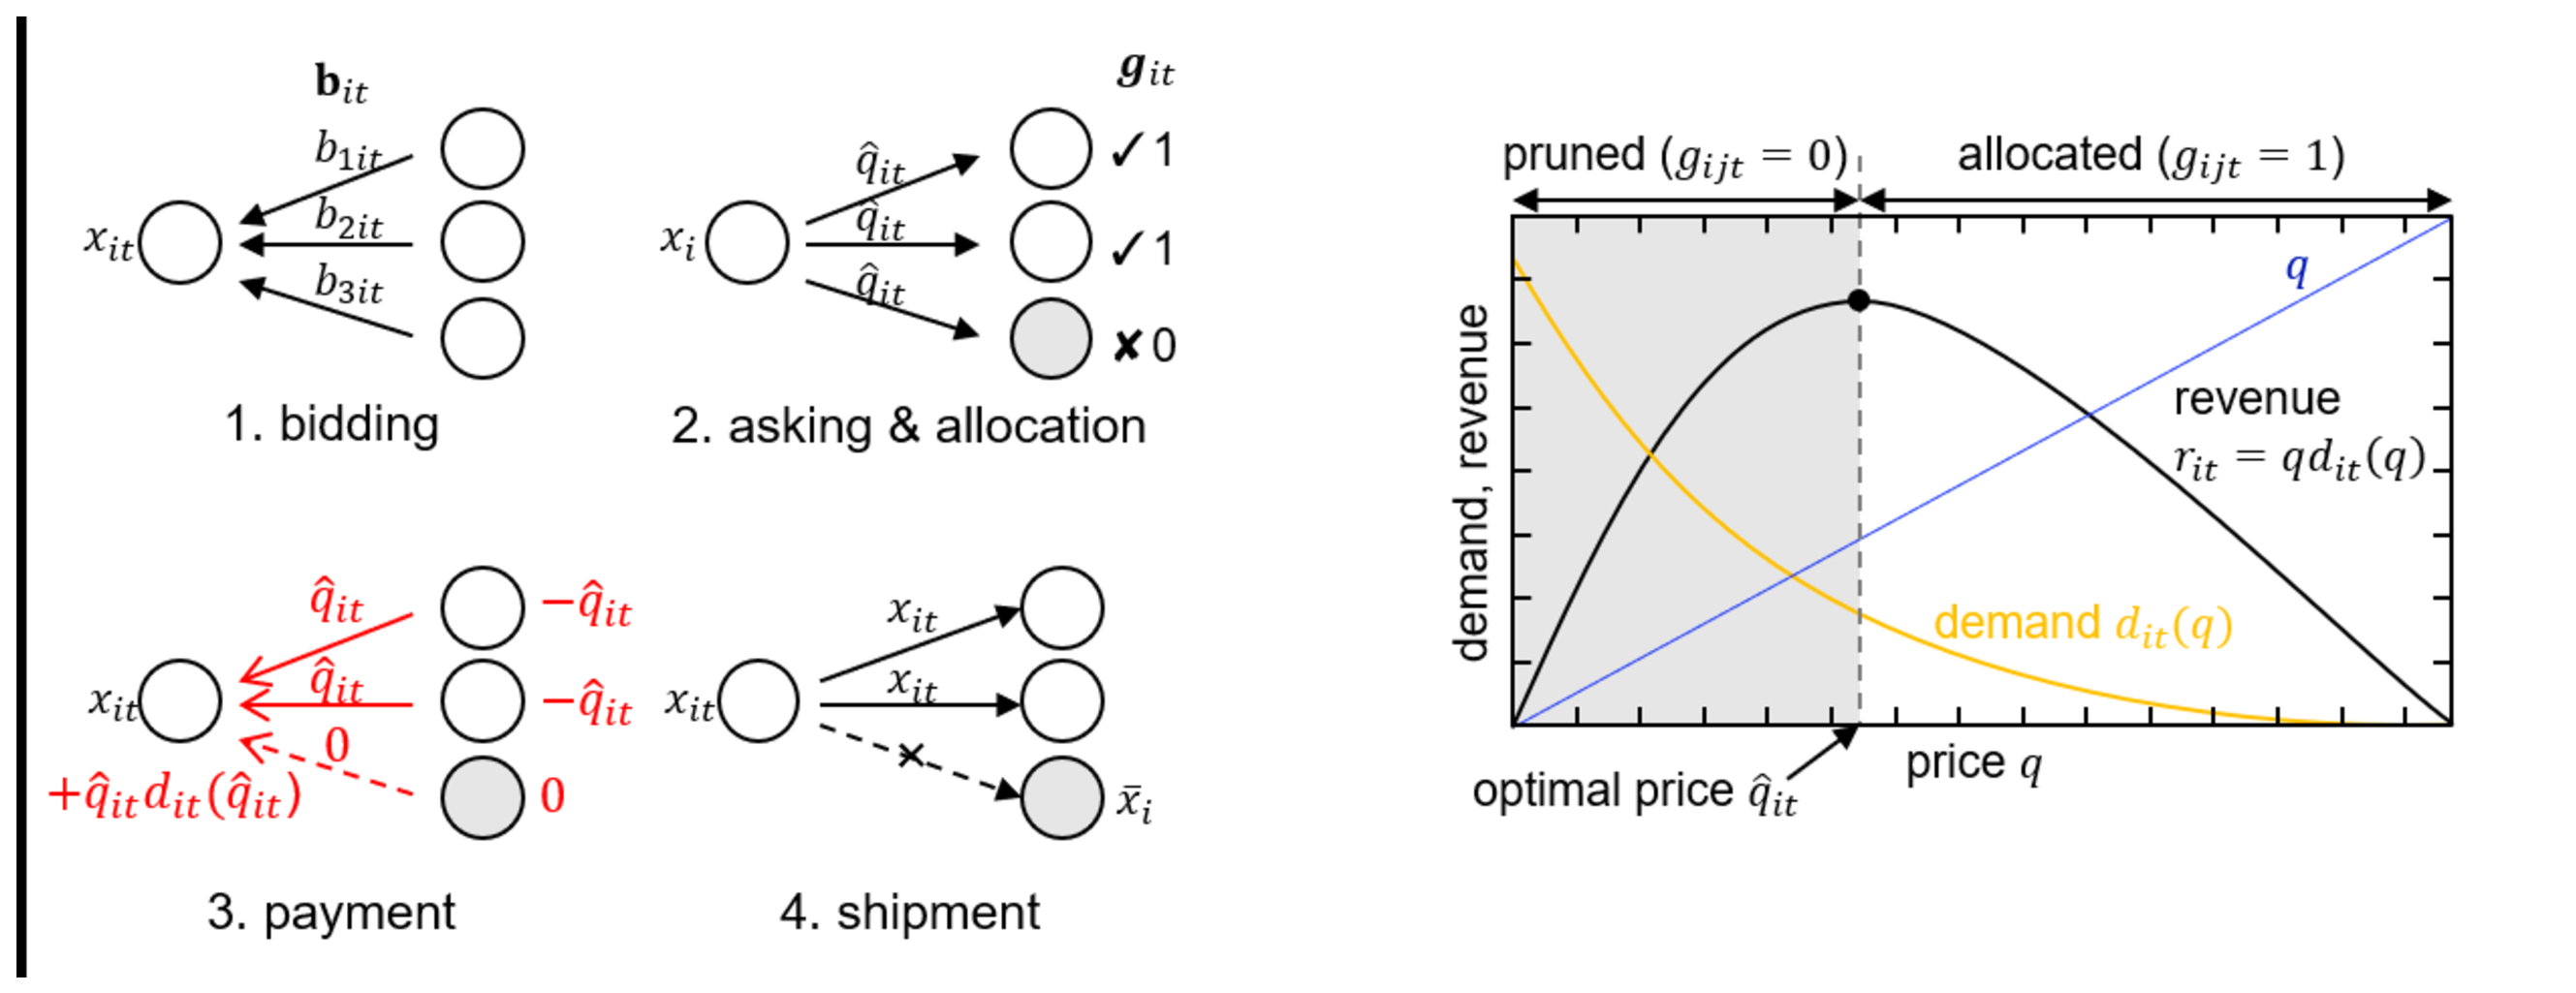
\includegraphics[width=\linewidth]{img/double.eps}
\caption{
Left: NaaA による取引の流れ。
Right: ユニットの価格決定方法。ユニットの収益は単調減少な需要と価格の積となり、これを最大化する価格が最適価格となる。
}
\label{fig:double}
\end{figure*}

% TODO 割当の話
Envy-free auction の流れを Figure \ref{fig:double} の左に示す。
図は、信号を送信する一つのユニットと、その信号を「購入」する複数のユニットに分かれ、交渉の過程を示している。
一単位の交渉は、強化学習の時間軸では 1 ステップ内に完了し、これが複数回繰り返されることになる。
信号を送信する側を売り手、受信する側を買い手と呼ぶ。
買い手はユニットに対して入札 $b_{jit}$ を行う(1)。次に、入札額をもとに、売り手は価格 $\opt{q}_{it}$ を決定し、割当を行う(2)。
このとき、$b_{jit} \ge \opt{q}_{it}$ であれば割当を行って $g_{jit} = 1$ とし、そうでなければ $g_{jit} = 0$ とする。
割当を行った後は、$\rho_{jit} = g_{jit} \opt{q}_{it}$ として、送金を行い(3)、
売り手は割当を行ったノードに対してのみ信号 $x_i$ を送付する(4)。
信号を受け取れなかったノードは、$x_i$ の期待値 $\Expect{\pi}{x_i}$ によって $x_i$ を近似する。
以下では、Envy-free auction における収益 $r_{it}$ とコスト $c_{it}$ の最適化について分けて説明を行う。

%この過程は、本や音楽などの、複製可能財、digital goods を対象にしたオークション理論 digital goods auction において、
%envy-free auction として知られている。
%後で示すように、このシンプルな前提のみでジレンマの問題が解決する。
%NaaA による取引の流れを図\ref{fig:double}に示す。

%========================================
% 収益
%========================================

\textbf{Revenue}:
エージェントの収益は次式で与えられる。
\begin{flalign}
	r_{it}  &= \sum_{j \in N^\mathrm{in}_i} g(b_{jit}, q_i) q_i + R^\mathrm{ex}_i  = q_i \sum_{j \in N^\mathrm{in}_i} g(b_{ji}, q_i)  + R^\mathrm{ex}_i \notag \\
		&= q_i d_t(q_t) + R^\mathrm{ex}_i
\end{flalign}
ここで、$a$ は価格、$d_t(a)$ はユニット $i$ の信号に対する価値を $a$ 以上と評価しているエージェントの数であり、需要(demand)と呼ぶ。
同様の式で、右辺を最大化する $a$ を最適価格と呼び、$ \opt{q}_{it} $ で表す。 
第二項は $q_t$ に対して独立であるから、最適価格 $\opt{q}_{it}$ は次のようにして与えられる。
\begin{flalign}
	\opt{q}_{it}  = \argmax_{q \in [0, \infty)} q d_{it}(q)
\end{flalign}
この仕組みを、Figure \ref{fig:double} の右に図示する。$d_t(q_{it})$ は単調減少な関数であり、$q_{it}$ との積によって表現される。


%========================================
% コスト
%========================================

\textbf{Cost}:
コストは、正しいデータを購入した場合とそうでない場合の期待リターン $G_{it}$ の差に等しい。
すなわち、
%FIXME 多分ここは期待値じゃなくてリターンそのものなのでそのように修正する(最初にリターンを使ったロジックで説明しているため)
\begin{flalign}
	o_t 
	&= \Expect{\pi}{ r_{i,t+1} \mid a_t=1 } - \Expect{\pi}{ r_{i,t+1} \mid a_t=0 } \notag \\
	&= \Expect{\pi}{ R_{i,t+1} \mid a_t=1 } - \Expect{\pi}{ R_{i,t+1} \mid a_t=0 } \notag \\
	&= Q(s_t, 1) - Q(s_t, 0) \label{eq:def:oppotunity-cost},
\end{flalign}
ただし、$Q$ は状態行動価値関数であり、一手先のコストはどちらの行動を選んでも一定であると仮定している。
$o_{it}$ を counterfractual state-action value と呼ぶ。これは QUICR \citep{agogino2006quicr} と導出は異なるが等価である。
すなわち、エージェントが支払うコストは、データの購入に成功した場合は $\opt{a}_{it}$ であり、
それ以外は $o_{it}$ となる。

では、コストを最小化するためのエージェントの入札額 $b_{it}$ は何か。
これについては次の定理が成立する。

\begin{thm}\label{thm:optimal-bidding}
コストを最小化する最適な入札額は $b_{it} = o_{it}$ である。
\end{thm}
証明については Appendix を参照。

すなわち、エージェントは自身の機会損失のみを問題にすればよい(!)
したがって、NaaA のメカニズムでは、エージェントはあたかも他のエージェントを価値評価(valuation)し、
その価値を正直に申告していることを意味する。

系として次の解が得られる。
\begin{coro}\label{coro:optimal-bidding}
The Nash equivalem of the envy-free game $(\vect{b}, q)$ is $(\vect{o}_t, \max_{q} q d_{\vect{o}_t}(q))$.
\end{coro}

%TODO o_t のグラウンドをする。最初に望ましい配分 v を述べ、その後で重要性について解説する。


\subsection{Valuation Net}

\begin{figure*}[t]
\centering
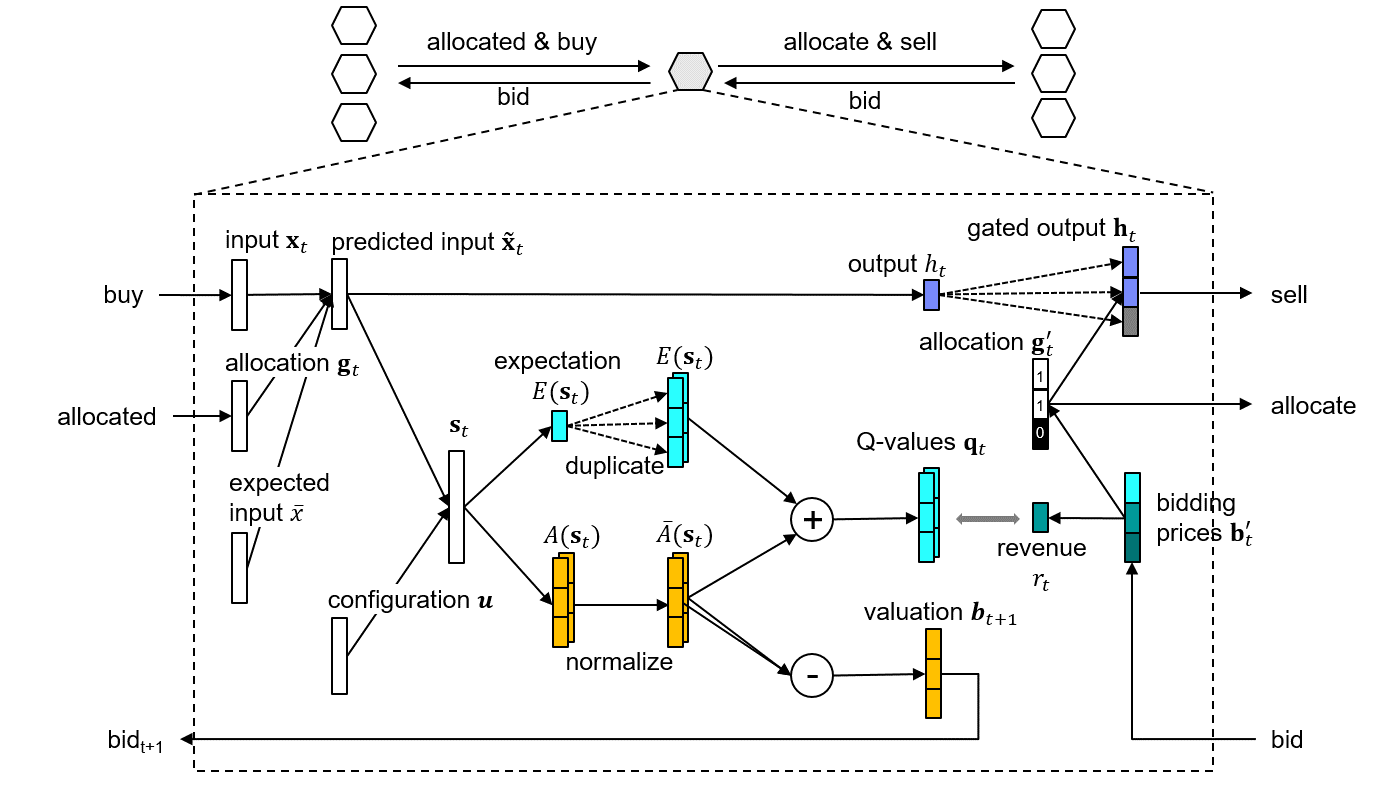
\includegraphics[width=\linewidth]{img/network.eps}
\caption{
Valuationn Net は情報の価値を評価し、bidding price を決定する。
下位のニューロンに対して入札し、信号を購入する。購入したデータを用いて、データを次のニューロンに対して売る。
}
\label{fig:network}
\end{figure*}

残る問題は、$\vect{o}_t$ をいかに推定するかである。
この推定には様々な方法が存在しており、多くのメソッドを使うことができるが、
本論文では $Q$ の推定に $Q$-learning を採用する。
ただし、SARSA や actor-critic などの on-policy な方法も使うことができることを補足する。

図\ref{fig:network}に示すValuation Net は、通常のニューラルネットワークのユニットに、
$Q$-learning による valuation を組み合わせたネットワークである。
まず、上部はエージェント間の通信について示したものである。
ニューラルネットワークではユニットを円で表現するのが通例であるが、
ここではユニットをエージェントとしてみなすことを強調して、六角形で一つのユニットを表現している。
エージェント間では、通常のニューラルネットワークと同様の信号の通信以外に、
取引に関する通信(allocate, buy, sell \& bid)が発生する。

Valuation Net では、状態 $\vect{s}_t$ として、
予測後入力 $\tilde{\vect{x}}_t$ および入力に依存しない構成情報 $\vect{u}$ を横につなげたベクトル $(\tilde{\vect{x}}_t^\T, \vect{u}^\T)^\T$ を用いる。
構成情報の一例としてはユニットのパラメータがあげられ、たとえば重みやバイアスの情報を用いることができる。

状態からの Q 関数の予測にニューラルネットワークを用いる。
エージェントが受け取った収益に基づき時間差分(TD)-誤差 が計算され、
ネットワークが訓練される。
ネットワークの構成にはこれまでの deep Q-learning で用いられている二重化ネットワーク(dualing network) \citep{wang2015dueling} のテクニックを用いる。
オリジナルの文献\citep{wang2015dueling}で述べられている二重化ネットワークは、学習を加速するために、
状態関数と、Q関数との差分を別々に予測する手法である。
\cite{dosovitskiy2016learning} はこれに対して、差分の要素の総和が 0 になるように正規化するよう改良している。
本研究では \cite{dosovitskiy2016learning} の手法に従い、
期待値 $\edges(\vect{s}_t)$ と正規化差分 $\tilde{A}(\vect{s}_t)$ を別々に求める。

$Q$関数は次のように表現される。
\begin{flalign}
	Q(\vect{s}_t, a_t) &= \edges(\vect{s}_t) + \tilde{A}(\vect{s}_t, a_t) \label{eq:QisE-A} \notag \\
	\sum_{i+1}^k \tilde{A}_i(\vect{s}_t, a_t) &= 0
\end{flalign}
第2式を満たすために、まず、$\vect{s}_t$に基づいた予測を行い、次のような正規化を行う。
\begin{flalign}
	\tilde{A}_i(\vect{s}_t, a_t) &= A_i(\vect{s}_t, a_t)  - \frac{1}{k} \sum_{j=1}^k  A_j(\vect{s}_t, a_t)
\end{flalign}
次に、valuation を行い、bidding price $\vect{b}_t$ を求める。
$b_{it}$ の値は式 \ref{eq:def:oppotunity-cost} および式 \ref{eq:QisE-A}より、最適な入札価格 $\opt{b}_{it}$ は次のように計算できる。
\begin{flalign}
\opt{b}_{it} = \tilde{A}(\state_t, 1) - \tilde{A}(\state_t, 0)
\end{flalign}
Valuation Net ではこの式に基づき、advantage の出力を引き算することで入札価格を計算している。


%\subsection{Valuation Net}

% method

\section{Experiment}
To confirm that NaaA works widely with machine learning tasks, we confirm our method of supervised
learning tasks as well as reinforcement learning tasks. As supervised learning tasks, we use
typical machine learning tasks such as image classification using MNIST, CIFAR-10, and SVHN.

As reinforcement tasks, we confirm single- and multi-agent environment. The single-agent environment
is from OpenAI Gym. We confirm the result using a simple reinforcement task: CartPole. In
multi-agent, we use ViZDoom, a 3D environment for reinforcement learning.

\subsection{Classification}
\subsubsection{Setup}
%This experiment verified the performance of two tasks: classification and single-agent reinforcement learning.
For classification, three types of datasets were used: MNIST, CIFAR-10, and STL-10. 
The given task was to predict the label of each image, and each dataset had a class number of 10.
The first dataset, MNIST, was a collection of black and white images of handwritten digits sized 28�~28. The training and test sets contained 60,000 and 10,000 example images, respectively. 
The CIFAR-10 dataset images were colored and sized 32�~32, and the assigned task was to predict what was shown in each picture. This dataset contained 6,000 images per class (5,000 for training and 1,000 for testing).
The STL-10 dataset was used for image recognition, and had 1,300 images for each class (500 training, 800 testing). Each image was sized 96�~96; however, for the experiment, the images were resized to 48�~48 because the greater resolution of this dataset (relative to the above datasets) required far more computing time and resources.

\subsubsection{Model}
Two models were compared in this experiment: DropConnect and Adaptive DropConnect (the model proposed in this paper). The baseline model was composed of two convolutional layers and two fully connected layers whose outputs are dropped out (we set the possibility as 0.5). The labels of input data were predicted using log-softmaxed values from the last fully connected layer. In the DropConnect and Adaptive DropConnect models, the first fully connected layer was replaced by a DropConnected and Adaptive DropConnected layer, respectively. It should be noted that the DropConnect model corresponded to the proposed method when $\varepsilon$ = 1.0, meaning agents did not perform their auctions but instead randomly masked their weights.

\subsubsection{Results}
The models were trained over ten epochs using the MNIST datasets, and were then evaluated using the test data. The CIFAR-10 and STL-10 epoch numbers were 20 and 40, respectively. Experiments were repeated 20 times for each condition, and the averages and standard deviations of error rates were  calculated. Results are shown in Table \ref{tbl:cls}. As expected, the Adaptive DropConnect model performed with a lower classification error rate than either the baseline or DropConnect models regardless of the given experimental datasets.


\begin{table}[h]
	\caption{ Experimental result for image classification tasks and single-agent RL }\label{tbl:cls}. 
\centering
\begin{tabular}{l|ccc|c}
\hline
		& MNIST & CIFAR-10 & STL-10 & CartPole \\
\hline
		DropConnect \citep{wan2013regularization}	&	1.72 $\pm$ 0.160	&	43.14 $\pm$ 1.335	&	50.92 $\pm$ 1.322 & 285 $\pm$ 21.5 \\
		Adaptive DropConnect	&	\textbf{1.36} $\pm$ 0.132	&	\textbf{39.84} $\pm$ 1.035	&	\textbf{42.17} $\pm$ 2.329 & \textbf{347} $\pm$ 29.4 \\
\hline
\end{tabular}
\end{table}

\subsection{Single-agent RL}
Next, the single-agent reinforcement learning task was set as 
the CartPole task from OpenAI Gym \citep{openaigym} with visual inputs.
In this setting, the agent was required to balance a pole while moving a cart.
The images contained a large amount of non-useful information, making pixel pruning important.
The result in Table \ref{tbl:cls} demonstrates that our method improves the standard RL.

\subsection{Multi-agent RL}
The proposed reward distribution method was confirmed to work as expected by a validation experiment using the multi-agent setting in ViZDoom \citep{kempka2016vizdoom}, 
an emulator of Doom containing a map editor where additional agents complement the main player.
A main player in the ViZDoom environment aims to seek the enemy in the map and then defeat the enemy.

\subsection{Setup}
A defend the center (DtC)-based scenario, provided by ViZDoom platform, was used for this experiment.
Two players, a main player and a cameraman, were placed in the DtC, where they started in the center of a circular field and then attacked enemies that came from the surrounding wall.
Although the main player could attack the enemy with bullets, 
the cameraman had no way to attack, only scouting for the enemy.
The action space for the main player was the combination of \{ attack, turn left, turn right \}, giving a total number of actions $2^3 = 8$.
The cameraman had two possible actions: \{ turn left, turn right \}.
Although the players could change direction, they could not move on the field.
Enemies died after receiving one attack (bullet) from the main player, and then player received a score of +1 for each successful attack.
The main player received 26 bullets by default at the beginning of each episode.
The main player died if they received attacks from the enemy to the extent that their health dropped to 0, and received a score of -1 for each death.
The cameraman did not die if attacked by an enemy.
Episodes terminated either when the maim player died or after 525 steps elapsed.

\subsection{Model}
Three models, described below, were compared: the proposed method and two comparison targets.

{\em Baseline}: DQN without communication. The main player learned standard DQN with the perspective that the player is viewing.
Because the cameraman did not learn, this player continued to move randomly.

{\em Comm}: DQN with communication, inspired by Commnet. The main player learns DQN with two perspectives: theirs and that of the cameraman.
The communication vector is learned with a feed-forward neural network.

{\em NaaA}: The proposed method. The main player learned DQN with two perspectives: theirs and that of the cameraman.
Transmissions of rewards and communications were performed using the proposed method.

\begin{figure*}[t]
\centering
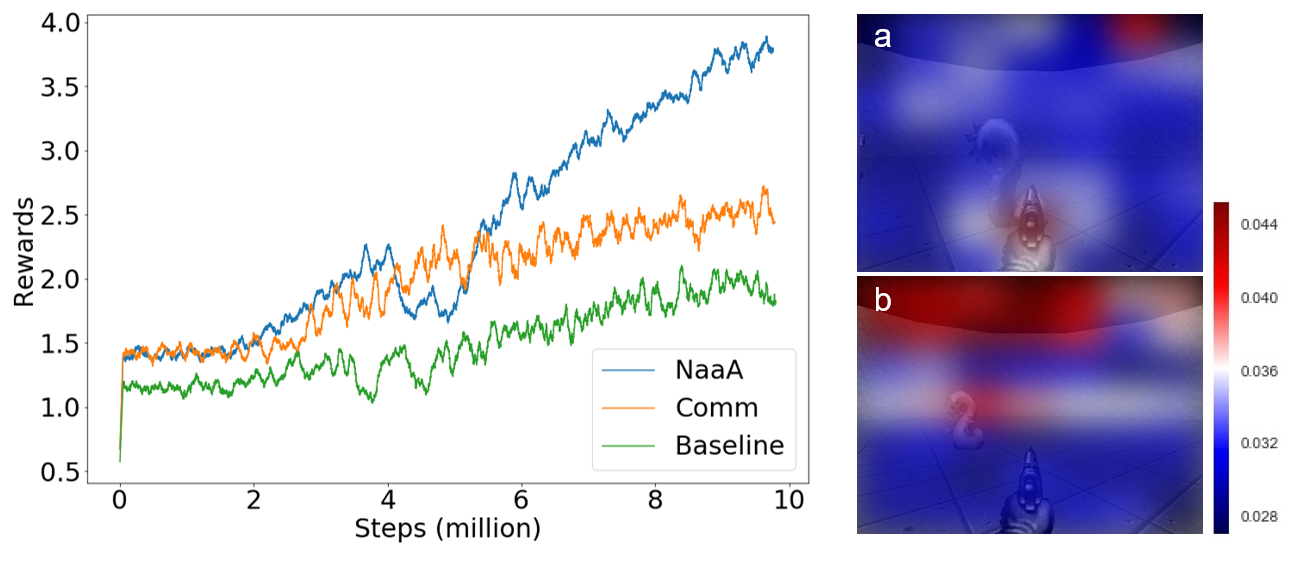
\includegraphics[width=\linewidth]{img/lc_vis.eps}
\caption{
	\textbf{Left:}
		Learning curve for ViZDoom multi-agent task. 
		The proposed NaaA--based method outperformed the other two methods (baseline and Comm DQNs).
	\textbf{Right:} 
		Visualizing reward from the main player to the cameramann shows us what is important information for the main player:
		(a) The pistol.
		(b) The point at which the enemy appeared and approached.
}
\label{fig:lc_vis}
\end{figure*}

\begin{figure*}[t]
\centering
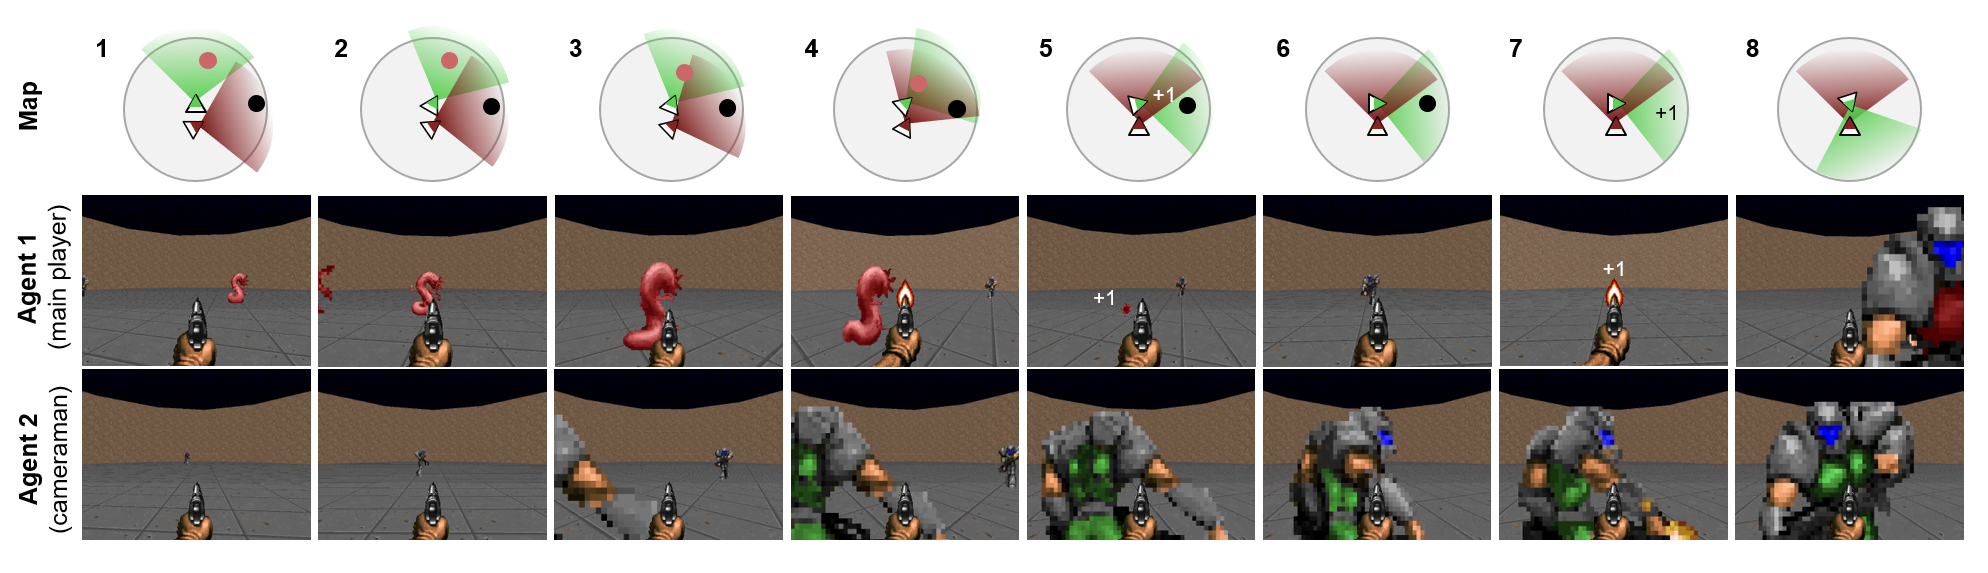
\includegraphics[width=\linewidth]{img/circleworld.eps}
\caption{
NaaA leads agents to enter a cooperative relationship.
First, the two agents face different directions,
and the cameraman sells their information to the main player (\textbf{1}).
The main player (information buyer) starts to turn right to find the enemy.
The cameraman (information seller) starts to turn left to seek new information by finding the blind area of the main player (\textbf{2} and \textbf{3}).
After turning, the main player attacks the first, having already identified enemy (\textbf{4} and \textbf{5}).
Once the main player finds the enemy, he attacks and obtains the reward (\textbf{6} and \textbf{7}).
Both agents then return to watching the dead area of the other until the next enemy appears (\textbf{8}).
}
\label{fig:circleworld}
\end{figure*}

\subsection{Results}
Training was performed over the course of 10 million steps.
Figure \ref{fig:lc_vis} Left demonstrates the proposed NaaA model outperformed the other two methods.
Improvement was achieved by Adaptive DropConnect.
It was confirmed that the cameraman observed the enemy through an episode, which could be interpreted as the cameraman reporting enemy positions.
In addition to seeing the enemy, the cameraman observed the area behind the main player several times.
This enabled the cameraman to observe enemy attacks while taking a better relative position.

To further interpret this result, 
a heatmap visualization of revenue earned by the agent is presented in Figure \ref{fig:lc_vis} Right.
The background picture is a screen from Doom, recorded at the moment when the CNN filter was most activated.
%The center corresponds to a position with the enemy appearing far away.
%The top corresponds to a position with the enemy coming closer.
%(b) shows that the agent sees the pistol.
Figure \ref{fig:circleworld} shows an example of learnt sequence of actions by our method.


%To confirm that NaaA works widely with machine learning tasks,
%we confirm our method of supervised learning tasks as well as reinforcement learning tasks.
%As supervised learning tasks, we use typical machine learning tasks such as image classification
%using MNIST, CIFAR-10, and SVHN.

%As reinforcement tasks, we confirm single- and multi-agent environment.
%The single-agent environment is from OpenAI gym.
%We confirm the result using a simple reinforcement task: CartPole.
%In multi-agent, we use ViZDoom, a 3D environment for reinforcement learning.

%The additional feature of NaaA is credit assignment for reward distribution, 
%meaning that if the neural network is divided into multiple agents, it works by playing the auction game.


\section{Discussion}
\subsection{Disadvantage}
Disdvantage としてまず挙げられるのは計算量である。
Envy-free auction では需要の計算にソートの演算が入るために、
直列化しなければならない箇所があるため、
これらについては近似を行うなどして改善していく必要がある。

個別の最適化技術について述べると、
Envy-free auction は、買い手のエージェント同士の価格がわからない sealed な状態であれば、
正直性(truthfulness)が成り立つが、一方で買い手同士がコミュニケーションを行い
価格を共有し合う状態においては、買い手が自由に価格を偽装できることが知られている。
これについては、によって解決方法が示されている。

Valuation Net は、用いるニューラルネットワークによっては実装が困難であることがある。
これは著者らの GitHub に Linear と CNN は公開しているが、
RNN などについては今後の研究課題となる。

\subsection{Application}
NaaA は、ネットワークが分散されている環境での学習や、サブモジュールでの制御に有用である。
具体的に、以下の技術に応用が可能である。

\begin{itemize}
\item ハイパーパラメータチューニング。Neuroevolution など、遺伝的アルゴリズムを用いてハイパーパラメータチューニングを用いるアルゴリズムがすでにいくつか提案されている。このとき、fitness 関数として利益を用いることで、より強化学習の目的に特化したニューラルネットワークを得ることができると考えられる。
\item アテンション制御。一部のアテンションの研究では、強化学習を用いてアテンションの制御を行っている。
\item アンサンブル。複数のモデルの混合に今回の技術を用いることができる。
\end{itemize}


\if0
(作成中)以下のトピックについて言及

何を観測するか考えるという意味合いにおいてはアテンションの拡張である

送金方法

通信スピードの問題

実際の POMDP への拡張

実装

オークションの competitive 性

\subsection{NaaA における「付加価値」とは何か}
具体的な付加価値の例は、統合( $\vect{w}^\T \vect{x}$ )、増幅・減衰( $cx$ )、整流( $\mathrm{ReLU}(x)$ )、バイアス ($x+b$) などである。

\subsection{信頼との関係}
\subsection{価値評価・買い物との関係}

\subsection{Disadvantage}
計算量の問題がある。

\subsection{アプリケーション}
NaaA は、分散環境で何かやったり、サブモジュールで何かコントロールするような場合に有用である。

・ハイパーパラメータチューニング(遺伝的アルゴリズムを用いてハイパーパラメータをチューニングする)
	・Neuroevolution。報酬系が fitness を決める。
・自己組織化ニューラルネットワーク
・アテンション制御
・アンサンブル法
\fi


\if0
想定される反論
・本質コストや NOOP の存在は、パレート劣位の証左にならない: オークションを使わなくても、最低コストだけ払えばよいのでは?
・
\fi


\section{Conclusion and Future Works}
�{�_���ł́APOMDP �̖��ݒ�ɂ����ėǎ��ȓ����\���𓾂邽�߂ɁA�j���[�����l�b�g���[�N��̊e���j�b�g���G�[�W�F���g�Ƃ��Ĉ����t���[�����[�N�ANaaA �ɂ‚��ďq�ׂ��B
NaaA �̃t���[�����[�N�ł́A�W�����}�����������A���ꂼ��̃G�[�W�F���g�̎��•t�����l���i�b�V���ύt�Ƃ��ē����A�S�̂Ƃ��ăp���[�g�œK�ɂȂ邱�Ƃ��������B
���D���i�̌���A���S���Y���̈�‚Ƃ��āA$Q$-learning �Ɋ�Â��l�b�g���[�N Valuation Net ���������B
�]�������ł́AAtari �� VizDoom ��p�����������s���A�������ʂ�������@�����悭�Ȃ邱�Ƃ��������B

% ����̕������͎v���‚����珑�������Ă���
����̕������Ƃ��āA�������AValuation Net �� A3C �Ȃǂ� on-policy �Ȏ�@�Œu��������Ƃ������������̑��A�_�o�Ȋw�I�Ȑ������”\�ɂ��Ă����Ƃ��������@�A��`�I�A���S���Y���Ƃ̑g�ݍ��킹����������B

\appendix
\section*{Appendix}

% Set numbering of section alphabet: A, B, C,...
\setcounter{section}{1}
\renewcommand{\thesection}{\Alph{section}}

% Contents is started from here
%\subsection{Proof}
%We first proof $\rho_{ijt} = 0$ is the Nash equilibrium.
%The value function can be written as $r_{it} - c_{it} + \gamma V_{i,t+1}$.
%At the point, as other agents plays $\rho_{ijt} = 0$, the value function is $- c_{it}$.
%To maximizing this equation, $\rho_{ijt} = 0$ holds. 

\subsection{Proof of Theorem \ref{thm:optimal-bidding}}
As for a buyer, the asking price $\ask$ for a seller is unknown,
we address $\ask$ which has support $[0, \infty)$,
and consideration to maximize $\Expect{q}{G(b,q)}$,
In this case, the following equation holds.
\begin{flalign}
\deriv{b}{}\Expect{q}{G(b,q)} 
&= \deriv{b}{}\int_0^\infty (H(b - q) \cdot (v-q) + G_0) p(q) dq \notag \\
&= \deriv{b}{} \left[ \int_0^b (v-q) p(q) dq + G_0 \int_0^\infty p(q)dq \right] \notag \\
&= \deriv{b}{} \int_0^b (v-q) p(q) dq \notag \\
&= (v-b) p(q=b), \notag 
\end{flalign}
Therefore, the condition to maximize $\Expect{q}{G(b,q)}$ is $b=v$.


\bibliography{daisy}
\bibliographystyle{iclr2017_conference}

\end{document}

